\documentclass{eecslides}
\usepackage{amsmath}

%------------------------------
% PAGE TITRE

\title[Forêts-CC]{Des changements abruptes à prévoir pour les forêts du Bas-St-laurent?}
\subtitle{Vers une nouvelle génération de modèles de dynamique forestière}
\author[D. Gravel]{Dominique Gravel}
\institute[Chaire de recherche EEC]{UQAR -- Chaire de Recherche EEC}
\website{http://www.chaire-eec.uqar.ca/}
\date{\today}

\begin{document}

%------------------------------

	\begin{frame}[plain]
		\titlepage
	\end{frame}
	
%-------------------------------------------------------------------------------
%-------------------------------------------------------------------------------
	\section{Introduction}
%-------------------------------------------------------------------------------
%-------------------------------------------------------------------------------

	\begin{frame}

		\textit{Les outils actuels pour prédire l'impact des changements climatiques sur les écosystèmes forestiers sont limités par l'absence de processus écologiques fondamentaux.}

	\end{frame}

%------------------------------

	\begin{frame}
		\begin{center}
				\begin{itemize}
					\item Où trouver du bois? Quelles essences?
					\item Quelle productivité?
					\item Quels sont les risques?			
				\end{itemize}
		\end{center}

	\end{frame}

%------------------------------

	\begin{frame}
		\begin{center}
			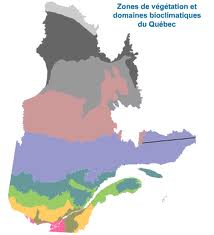
\includegraphics[height=0.75\textheight]{bioclim_MRN}
		\end{center}
	\end{frame}

%------------------------------

	\begin{frame}
		\begin{center}
			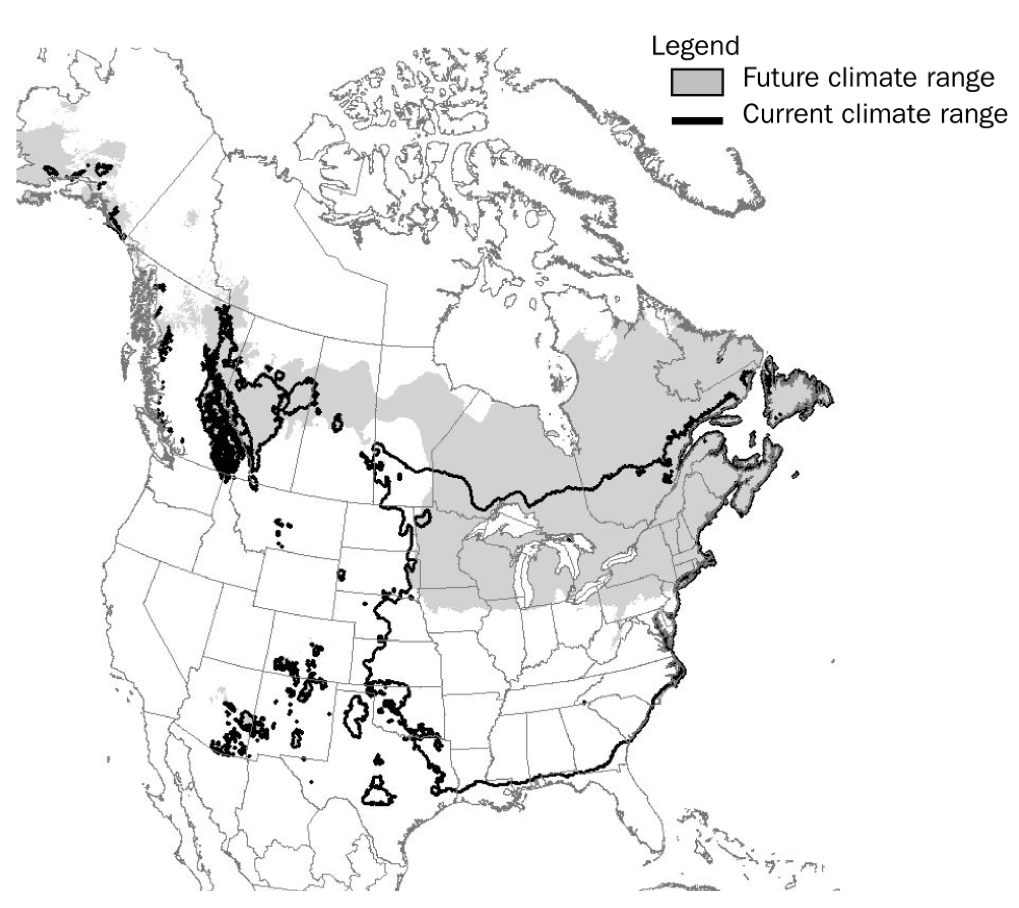
\includegraphics[height=0.65\textheight]{mckenney}
		\end{center}
	\end{frame}

%------------------------------

	\begin{frame}{Enveloppes climatiques}
		\begin{columns}
			\begin{column}{0.5\textwidth}
				\begin{center}
					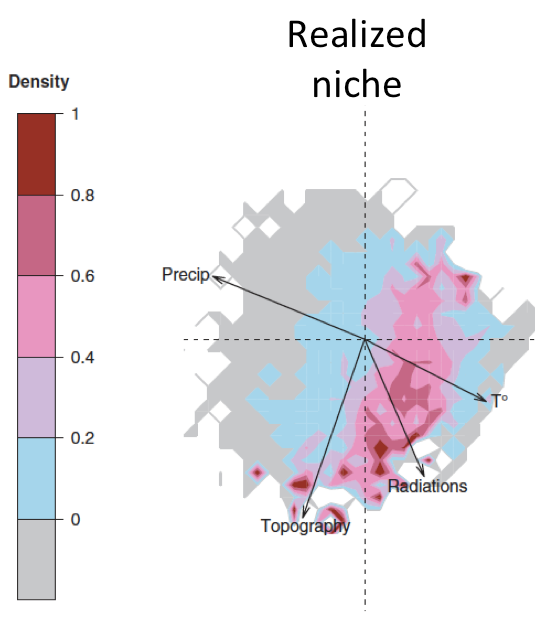
\includegraphics[height=0.5\textheight]{boulangeat}
				\end{center}
			\end{column}
%----
			\begin{column}{0.5\textwidth}
			De nombreuses suppositions
				\begin{itemize}
					\item Distribution à l'équilibre avec le climat;
					\item Aucune démographie;
					\item Aucune interaction biotique;
					\item Aucune limite à la dispersion;
					\item Réponse linéaire et instantanée au changement climatique;					
				\end{itemize}
			\end{column}
		\end{columns}	    	
	\end{frame}

%------------------------------

	\begin{frame}{Croissance et climat}
		\begin{center}
			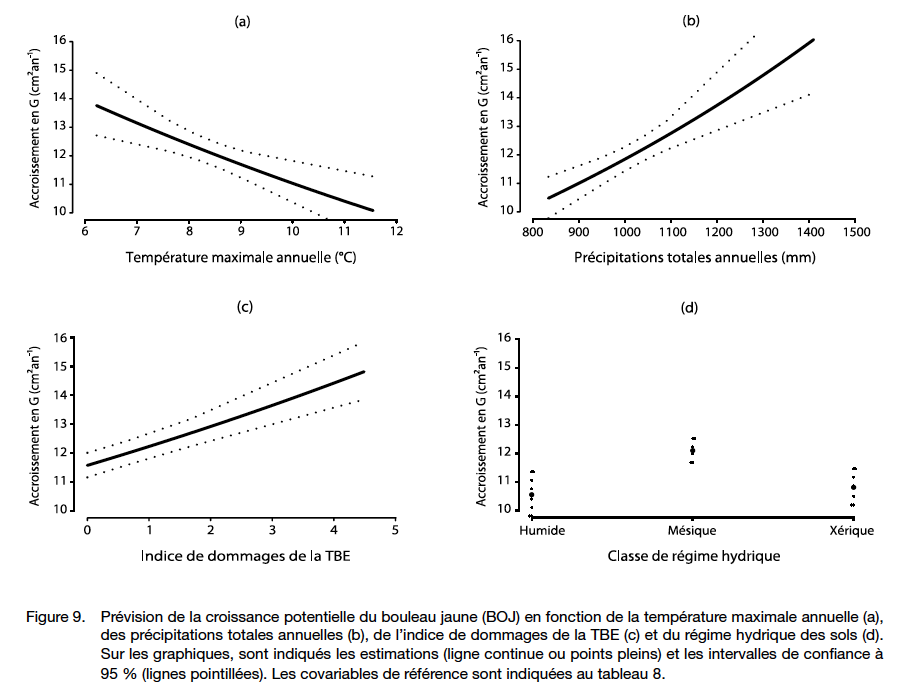
\includegraphics[height=0.65\textheight]{Perie2012.png}
		\end{center}
	\end{frame}

%------------------------------

	\begin{frame}{Objectifs}

		\textbf{Objectif général}: Prédire les impacts à court et long terme d'un changement climatique sur l'état et la productivité des forêts de l'Est du Canada. 
		\vskip 3em

		\textbf{Objectifs spécifiques}: 
		\begin{enumerate} 

			\item Développer de nouveaux outils de modélisation pour améliorer les prédictions de l'impact des changements climatiques sur les écosystèmes forestiers;
			\item Développer de nouvelles aproches pour estimer les risques et incertitudes;
			\item Évaluer l'aptitude de différentes stratégies d'aménagement forestier à minimiser les impacts négatifs des changements climatiques. 

		\end{enumerate}
	\end{frame}

%-------------------------------------------------------------------------------
%-------------------------------------------------------------------------------
	\section{Théorie}
%-------------------------------------------------------------------------------
%-------------------------------------------------------------------------------
	
%	\begin{frame}{Contexte théorique}
%		\begin{center}
%		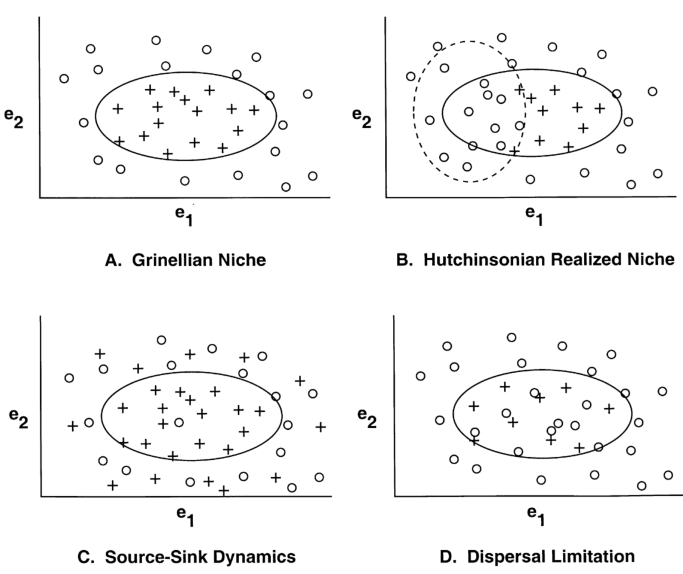
\includegraphics[height=0.6\textheight]{pulliam}\\
%		\end{center}
%	\end{frame}


%-------------------------------------------------------------------------------

%	\begin{frame}{Contexte théorique}
%		\begin{center}
%		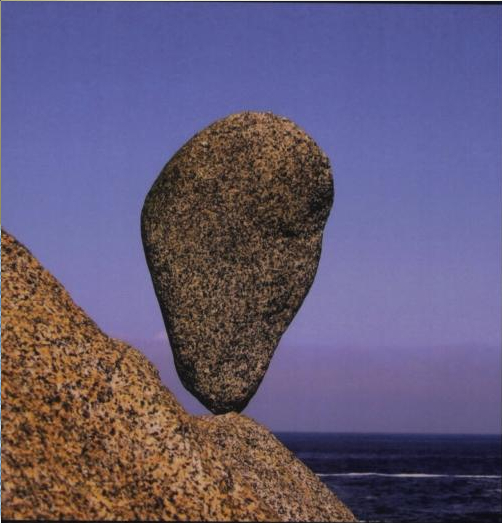
\includegraphics[height=0.6\textheight]{scheffer}\\
%		\end{center}
%	\end{frame}

%-------------------------------------------------------------------------------

	\begin{frame}{Quel type de transition?}
		\begin{center}
		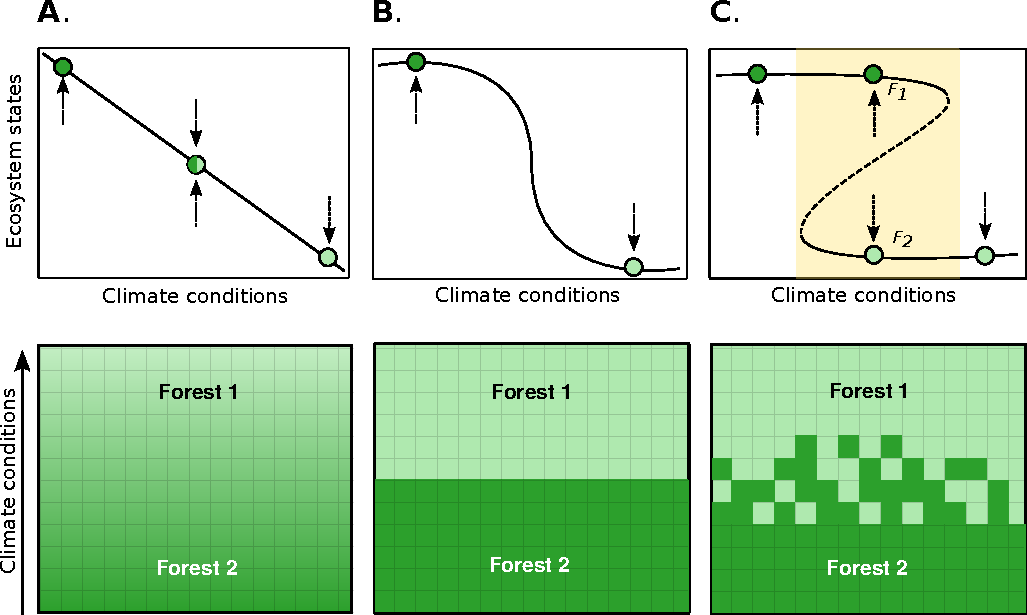
\includegraphics[height=0.6\textheight]{states}\\
		\end{center}
	\end{frame}

%-------------------------------------------------------------------------------

	\begin{frame}{Quel type de transition?}
		\begin{center}
		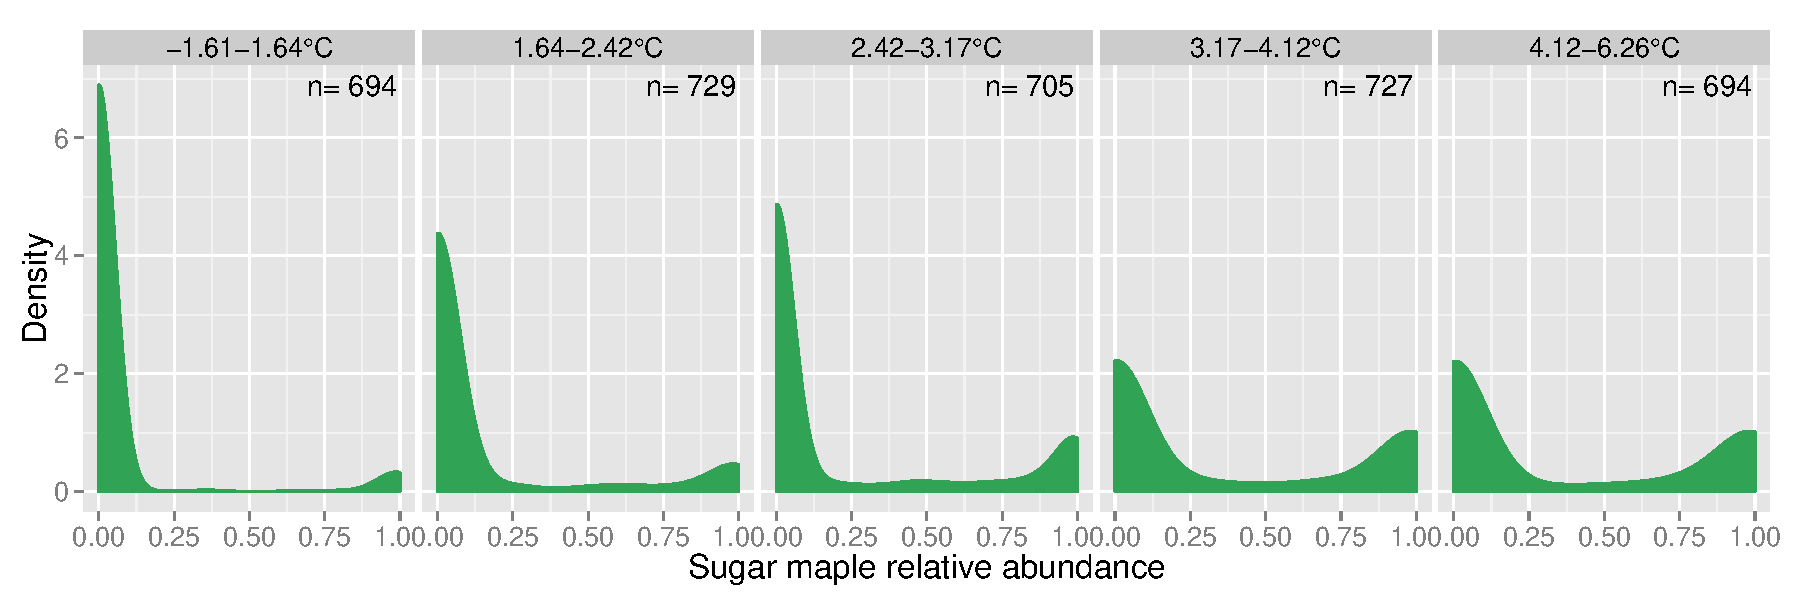
\includegraphics[height=0.4\textheight]{ass_ers}\\
		\end{center}
	\end{frame}

%%-------------------------------------------------------------------------------
%
%	\begin{frame}{Contexte théorique}
%		\begin{center}
%		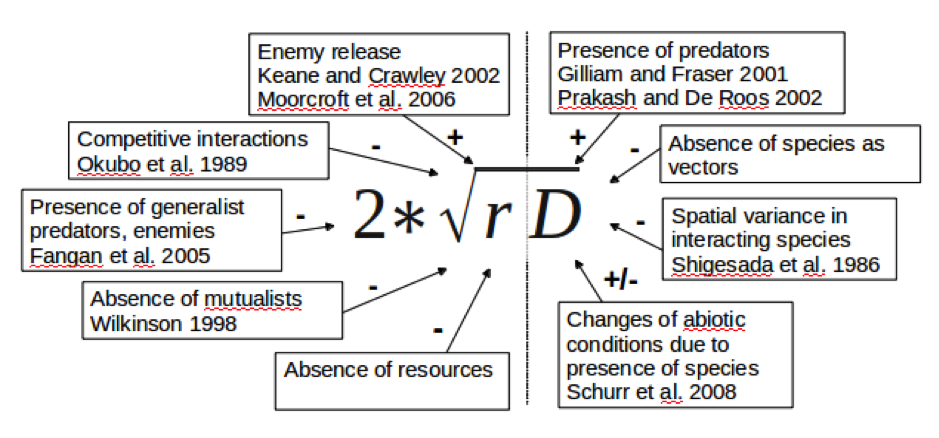
\includegraphics[height=0.6\textheight]{svenning}\\
%		\end{center}
%	\end{frame}

%%-------------------------------------------------------------------------------
%%-------------------------------------------------------------------------------
	\section{Projet}
%%-------------------------------------------------------------------------------
%%-------------------------------------------------------------------------------
%	
	\begin{frame}{Description du projet}{Volet 1}
		\textbf{Objectif}: Développer notre compréhension des facteurs qui affectent la migration des arbres sous l'effet des changements climatiques

		\begin{center}
			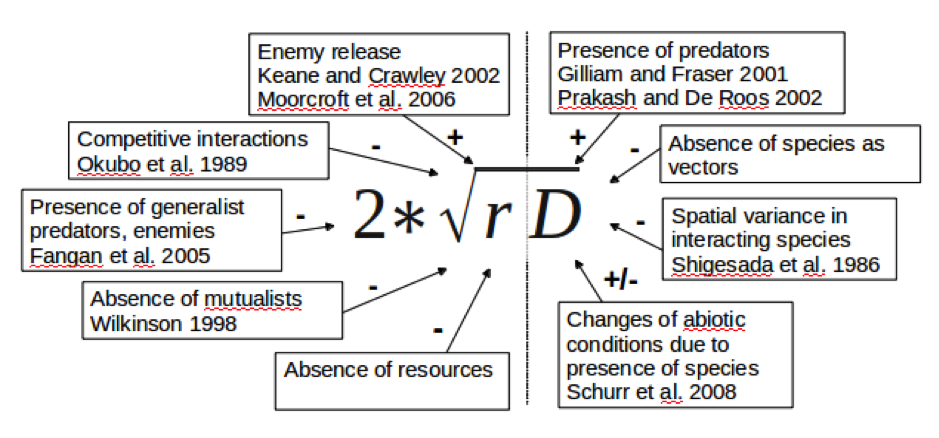
\includegraphics[height=0.5\textheight]{svenning.png}
		\end{center}

	\end{frame}
%
%%-------------------------------------------------------------------------------
	
	\begin{frame}{Description du projet}{Volet 2}

	\textbf{Objectif}: Développer des modèles démographiques dépendants du climat

		\begin{itemize}
			\item Croissance, mortalité et compétition;  
			\item Représenter spatialement les impacts à court terme sur la productivité;
			\item Tester si la diversité a un effet positif sur l'adaptation. 
		\end{itemize}
		
	\end{frame}

%-------------------------------------------------------------------------------
	
	\begin{frame}{Description du projet}{Volet 2}

		\begin{center}
			$Growth = MaxGrowth \times Interactions\times Size \times Climate $
		\end{center}
		
		\begin{center}
		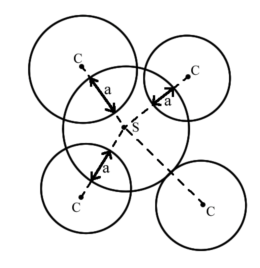
\includegraphics[height=0.4\textheight]{neighborhood}\\
		\end{center}
		
	\end{frame}

%-------------------------------------------------------------------------------	
	
	\begin{frame}{Description du projet}{Volet 3}
	\textbf{Objectif}: Développer une suite intégrée de modèles, de l'arbre jusqu'au continent 

		\begin{itemize}
			\item Modèle de peuplement dépendant du climat;
			\item Modèle de paysage dépendant du climat;
			\item Cartographie de la distribution et productivité future;
			\item Comparaison des taux de migration entre modèles;
			\item Couplage avec les espèces herbacées et les herbivores.
		\end{itemize}
	\end{frame}

%%-------------------------------------------------------------------------------
	
	\begin{frame}{Description du projet}{Volet 3}
		\begin{center}
		\includegraphics[height=0.6\textheight]{model_integration}\\
		\end{center}
	\end{frame}

%%-------------------------------------------------------------------------------
	\begin{frame}{Description du projet}{Volet 3}
		\begin{columns}
			\begin{column}{0.5\textwidth}
				\begin{center}
				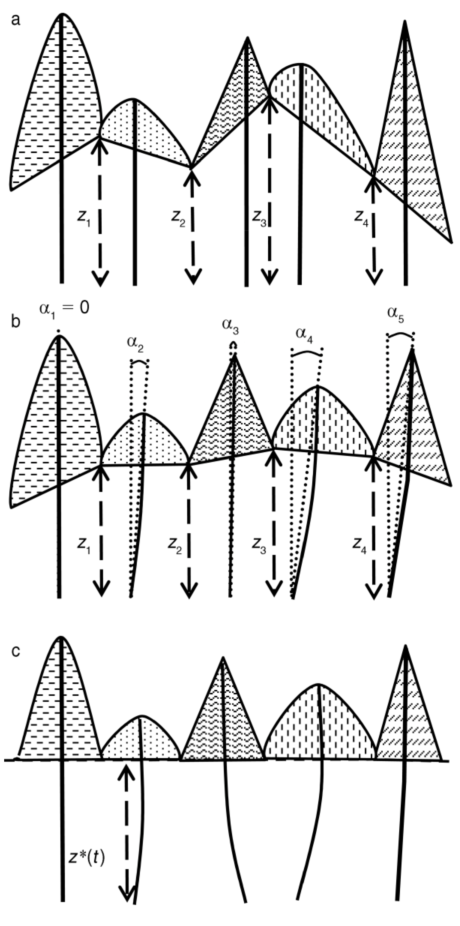
\includegraphics[height=0.6\textheight]{strigul}\\
				\end{center}	
			\end{column}
%----
			\begin{column}{0.5\textwidth}
				\begin{center}
				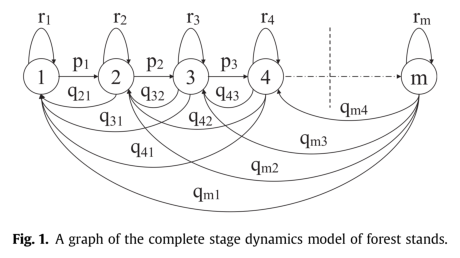
\includegraphics[height=0.3\textheight]{markov}\\
				\end{center}
			\end{column}
		\end{columns}	    	
	\end{frame}

%------------------------------		
	\begin{frame}{Description du projet}{Volet 4}

	\textbf{Objectif:} Évaluer de nouvelles stratégies d'aménagement forestier et de conservation

		\begin{itemize}
			\item Business as usual;
			\item Migration assistée;
			\item Couloirs de migration;
			\item Sylviculture haute diversité;
			\item Anticipation des changements de composition.	
		\end{itemize}
	\end{frame}

%-------------------------------------------------------------------------------
%-------------------------------------------------------------------------------
\section{Méthodes}
%-------------------------------------------------------------------------------
%-------------------------------------------------------------------------------
	\begin{frame}{Base de données}
		\begin{itemize}
			\item Parcelles échantillons temporaires (MRNQ);
			\item Parcelles échantillons permanentes (MRNQ)
			\item Domtar;
			\item OMNR;
			\item Nouveau-Brunswick;
			\item FIA.
		\end{itemize}
	\end{frame}

%-------------------------------------------------------------------------------

	\begin{frame}{Larges parcelles permanentes}
		\begin{columns}
			\begin{column}{0.35\textwidth}
			Mesures:
				\begin{itemize}
					\item Coordonnées des arbres;
					\item Diamètre;
					\item Espèce;			
					\item Regénération;
					\item Senseurs;
					\item Pièges fosse;
					\item Germination (expérience en parallèle sur 15 sites).
				\end{itemize}
			\end{column}	
%----				
			\begin{column}{0.65\textwidth}
				\begin{center}
					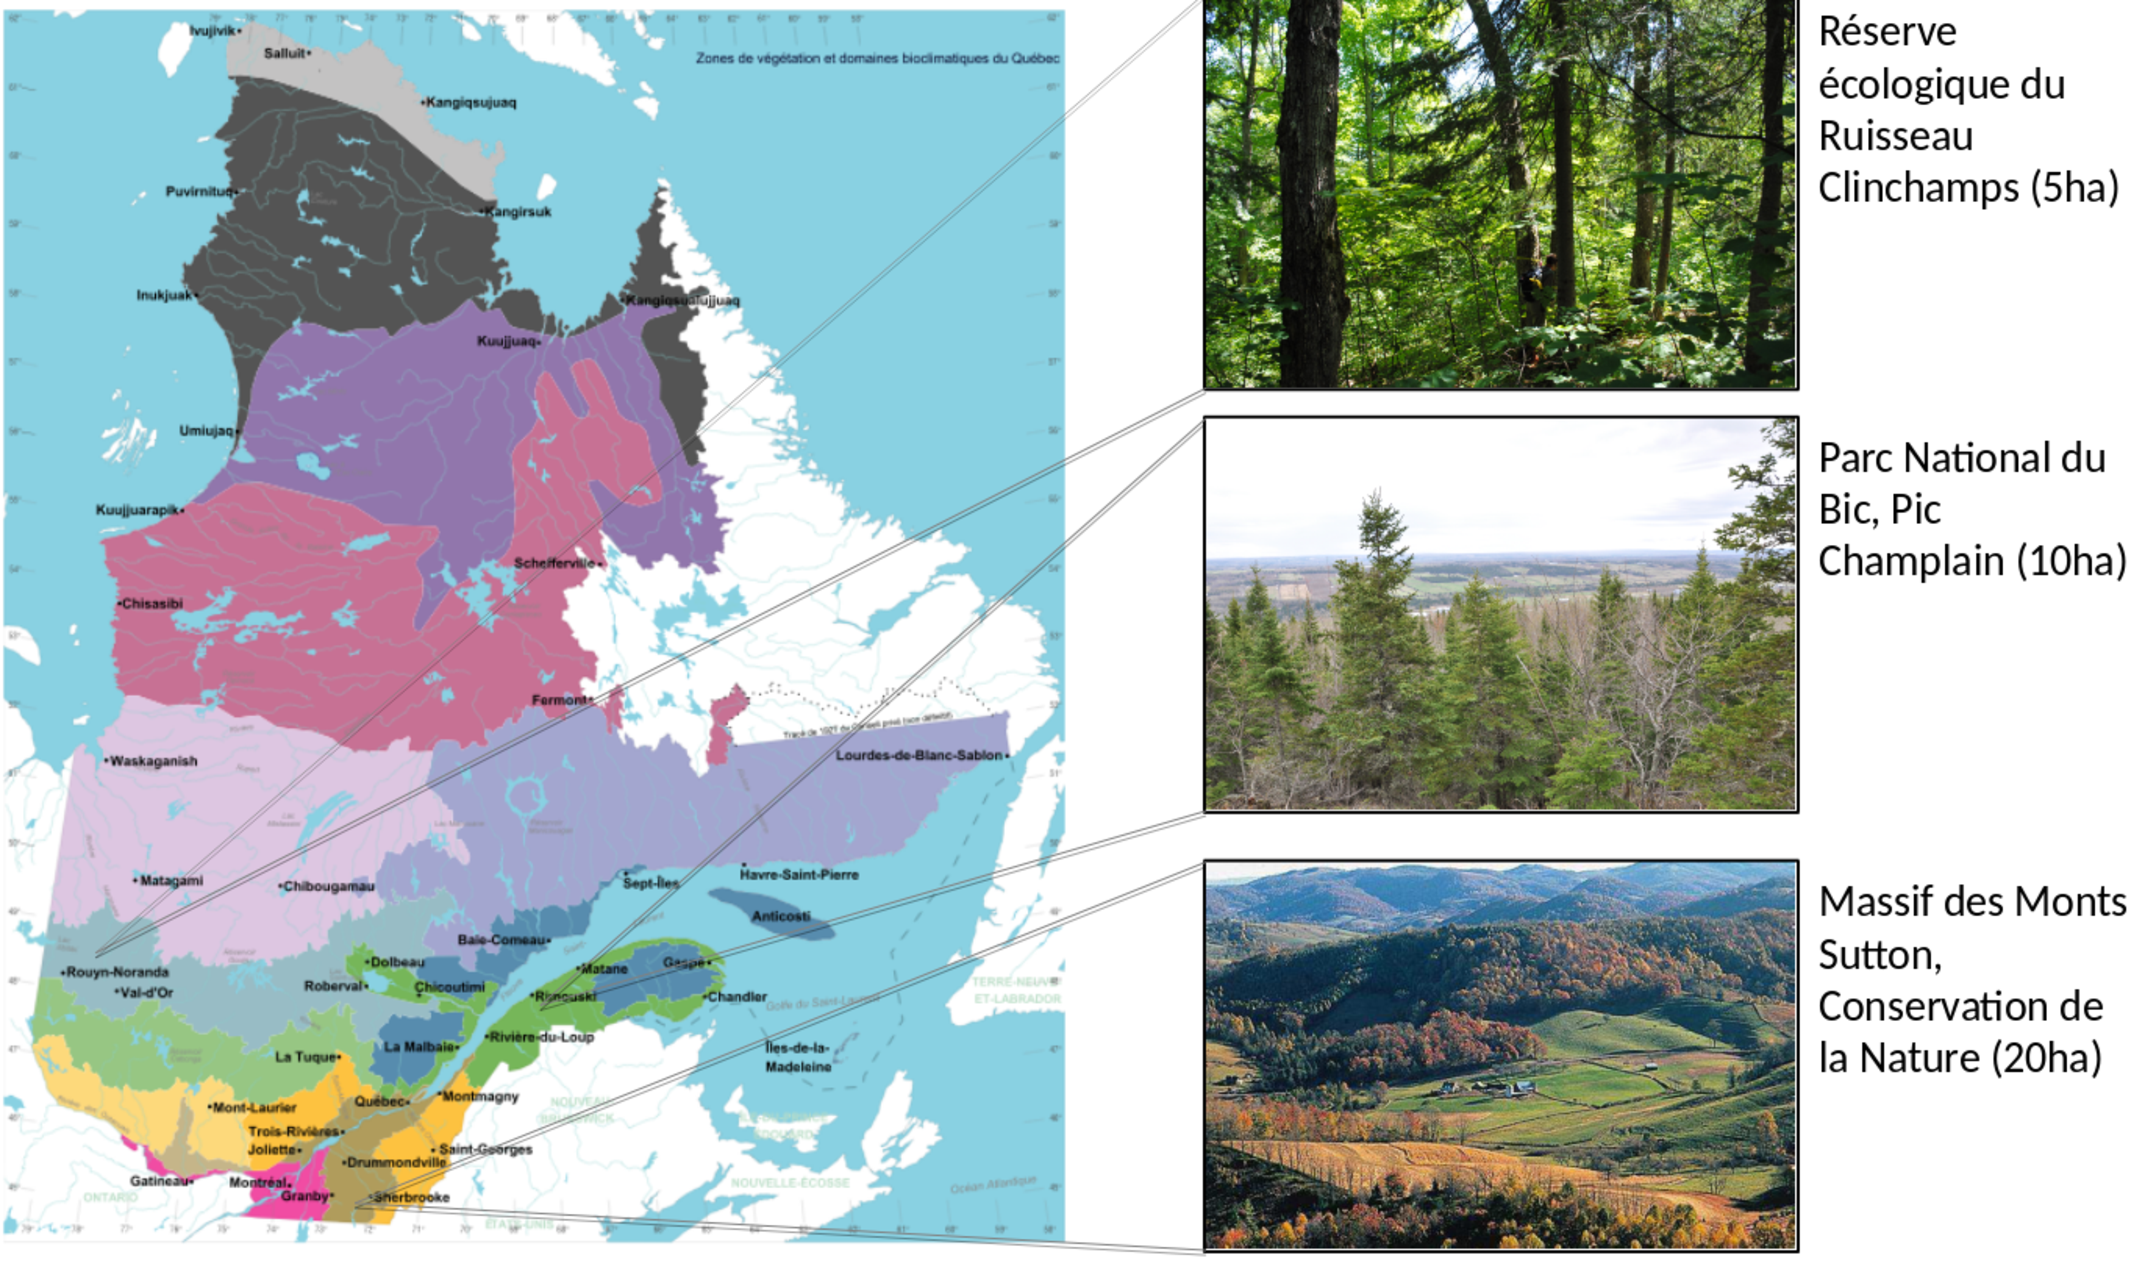
\includegraphics[height=0.5\textheight]{carte_parcelles}
				\end{center}
			\end{column}
		\end{columns}	    	
	\end{frame}

%-------------------------------------------------------------------------------

	\begin{frame}{Parcelle du Pic Champlain}
				\begin{center}
					\includegraphics[height=0.5\textheight]{carte_bic}
				\end{center}
	\end{frame}

%-------------------------------------------------------------------------------

	\begin{frame}{Parcelle du Pic Champlain}
		\begin{columns}
			\begin{column}{0.6\textwidth}
				\begin{center}
					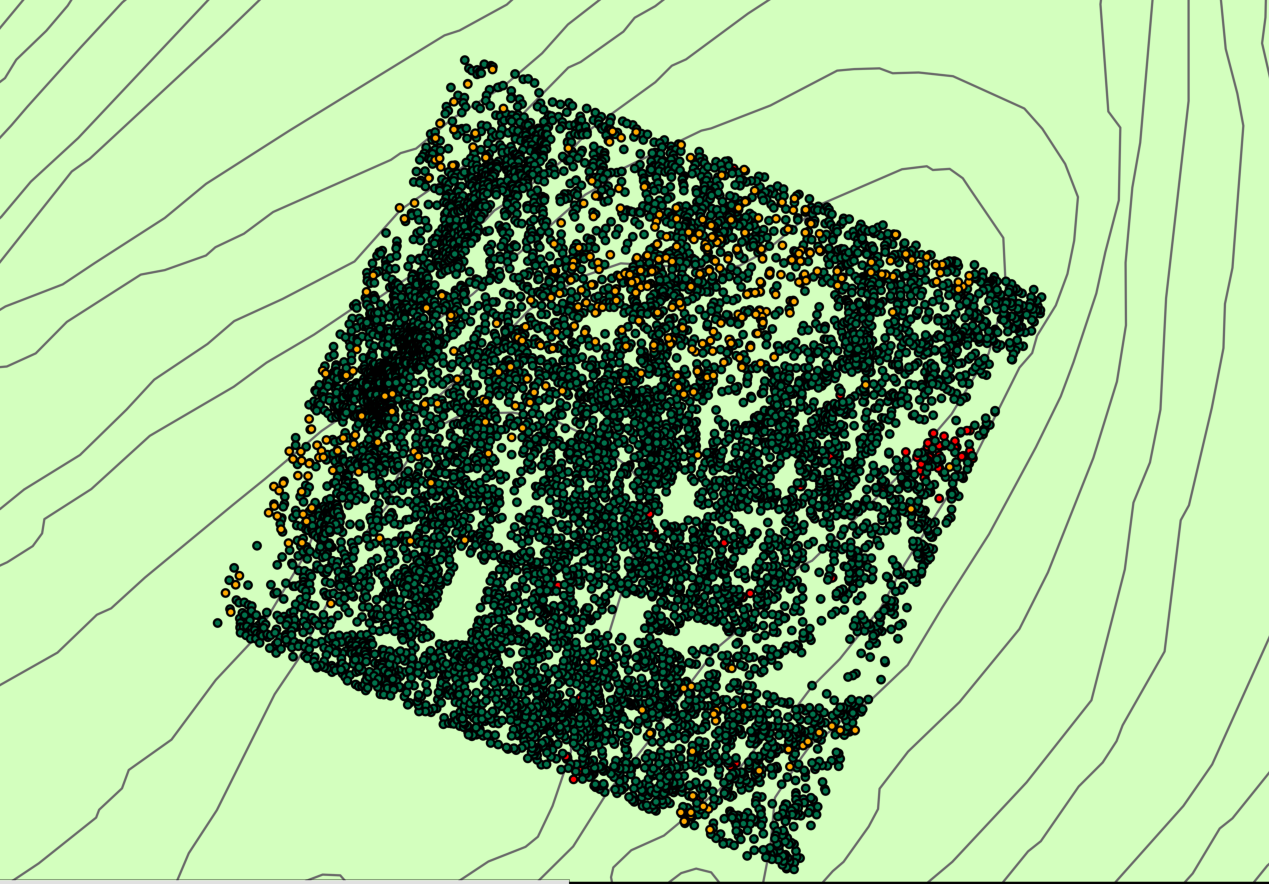
\includegraphics[height=0.5\textheight]{carte_arbres}
				\end{center}
			\end{column}
%----
			\begin{column}{0.4\textwidth}
				\begin{center}
					\includegraphics[height=0.5\textheight]{tableau_especes}
				\end{center}
			\end{column}
		\end{columns}	    	
	\end{frame}

%-------------------------------------------------------------------------------
%-------------------------------------------------------------------------------
\section{Exemple}
%-------------------------------------------------------------------------------
%-------------------------------------------------------------------------------


	\begin{frame}{Exemple}{Objectif}
		\begin{center}
			Prédire la distribution future de l'érablière en tenant compte de la démographie, de la succession et de la dispersion limitée.
		\end{center}
	\end{frame}

%-------------------------------------------------------------------------------

	\begin{frame}{Modèle}
		\begin{center}
			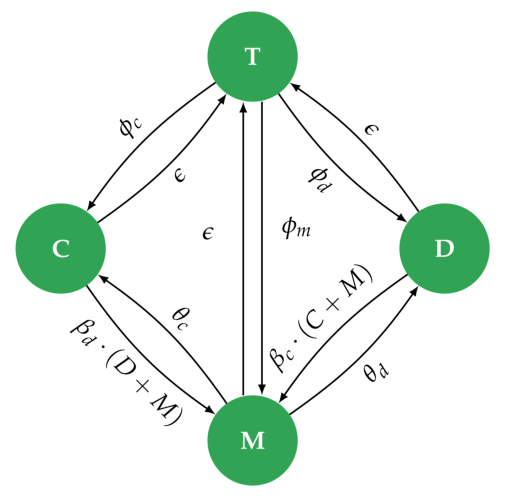
\includegraphics[height=0.6\textheight]{model}
		\end{center}
	\end{frame}

%-------------------------------------------------------------------------------

		\begin{frame}{Distribution}
		\begin{columns}
			\begin{column}{0.5\textwidth}
				Distribution actuelle des états
								\begin{center}
					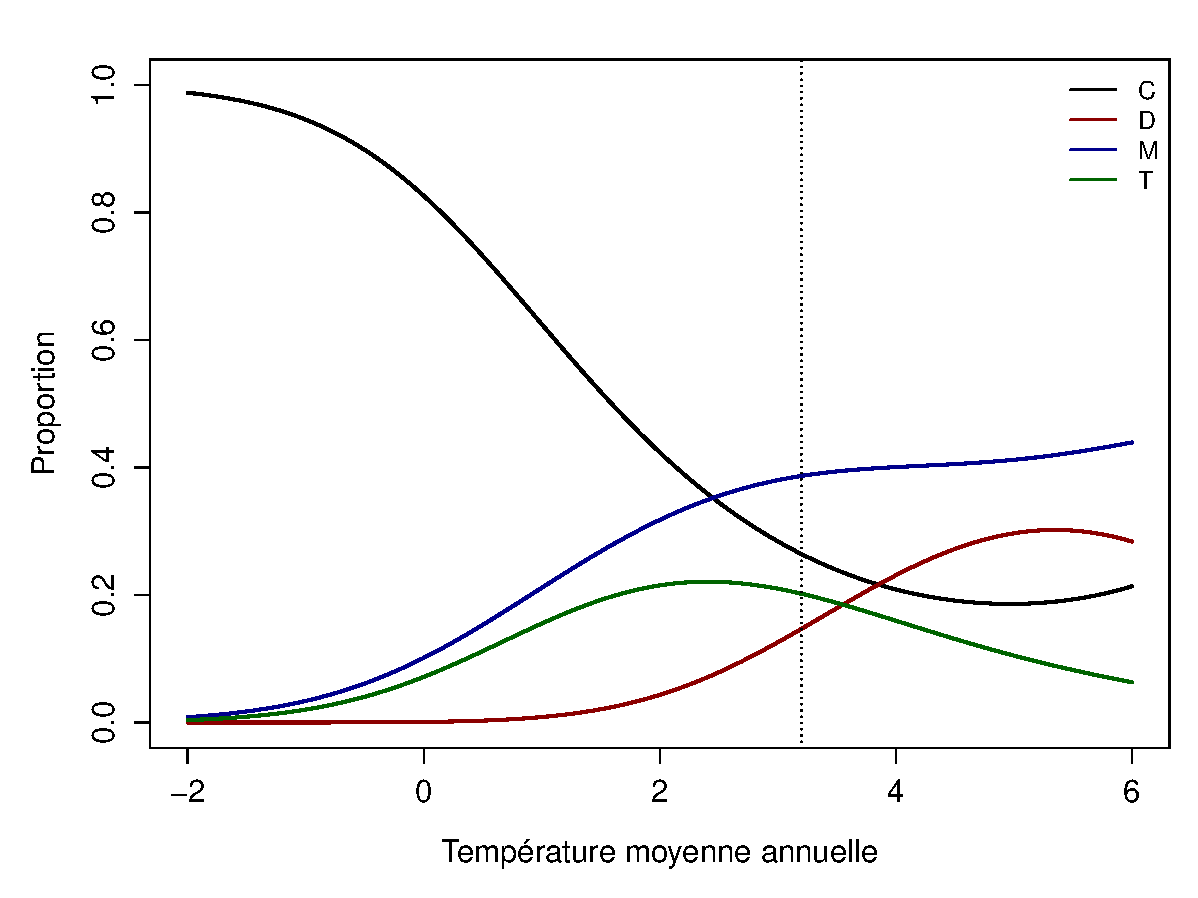
\includegraphics[height=0.4\textheight]{SDM}
				\end{center}
			\end{column}
%----
			\begin{column}{0.5\textwidth}
			\end{column}
		\end{columns}	    	
	\end{frame}

%-------------------------------------------------------------------------------

		\begin{frame}{Distribution}
		\begin{columns}
			\begin{column}{0.5\textwidth}
				Distribution actuelle des états
								\begin{center}
					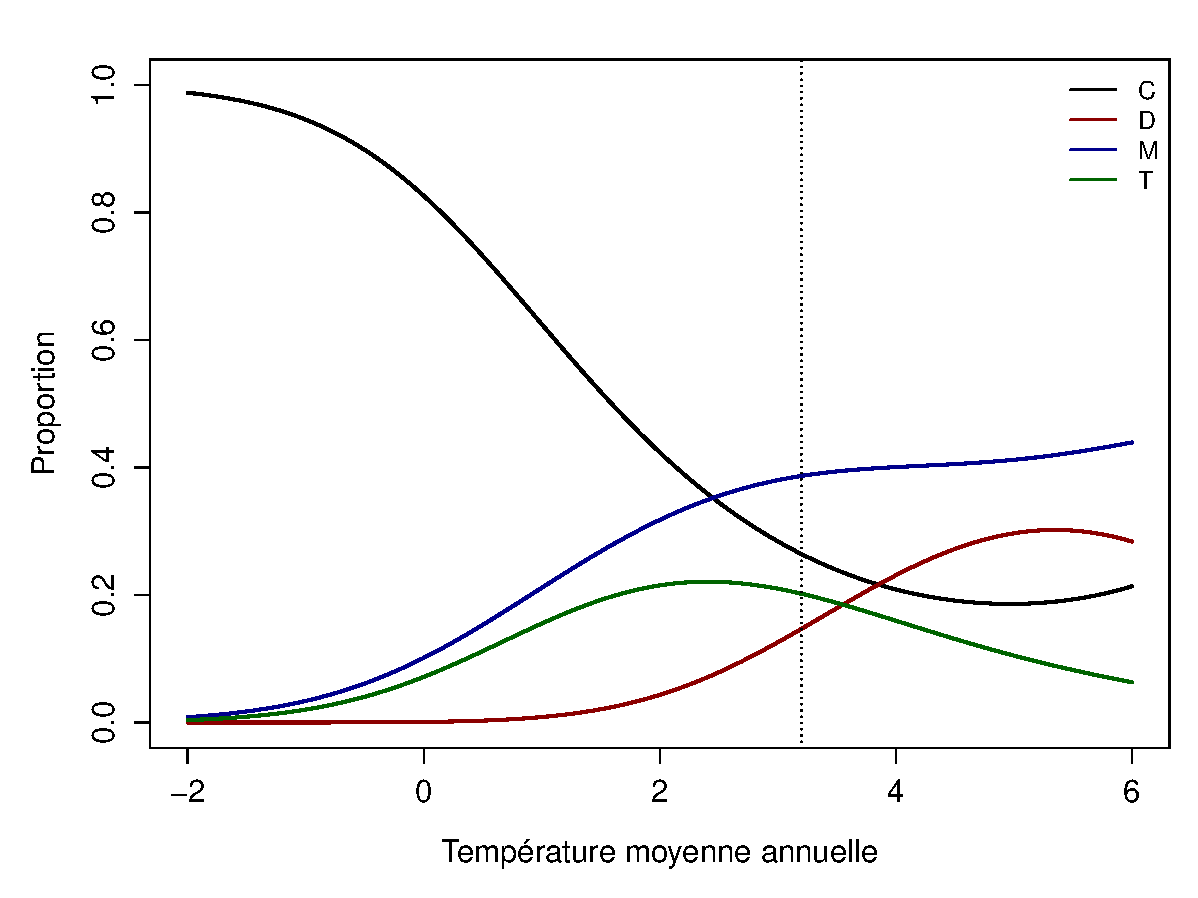
\includegraphics[height=0.4\textheight]{SDM}
				\end{center}
			\end{column}
%----
			\begin{column}{0.5\textwidth}
				Distribution modélisée
				\begin{center}
					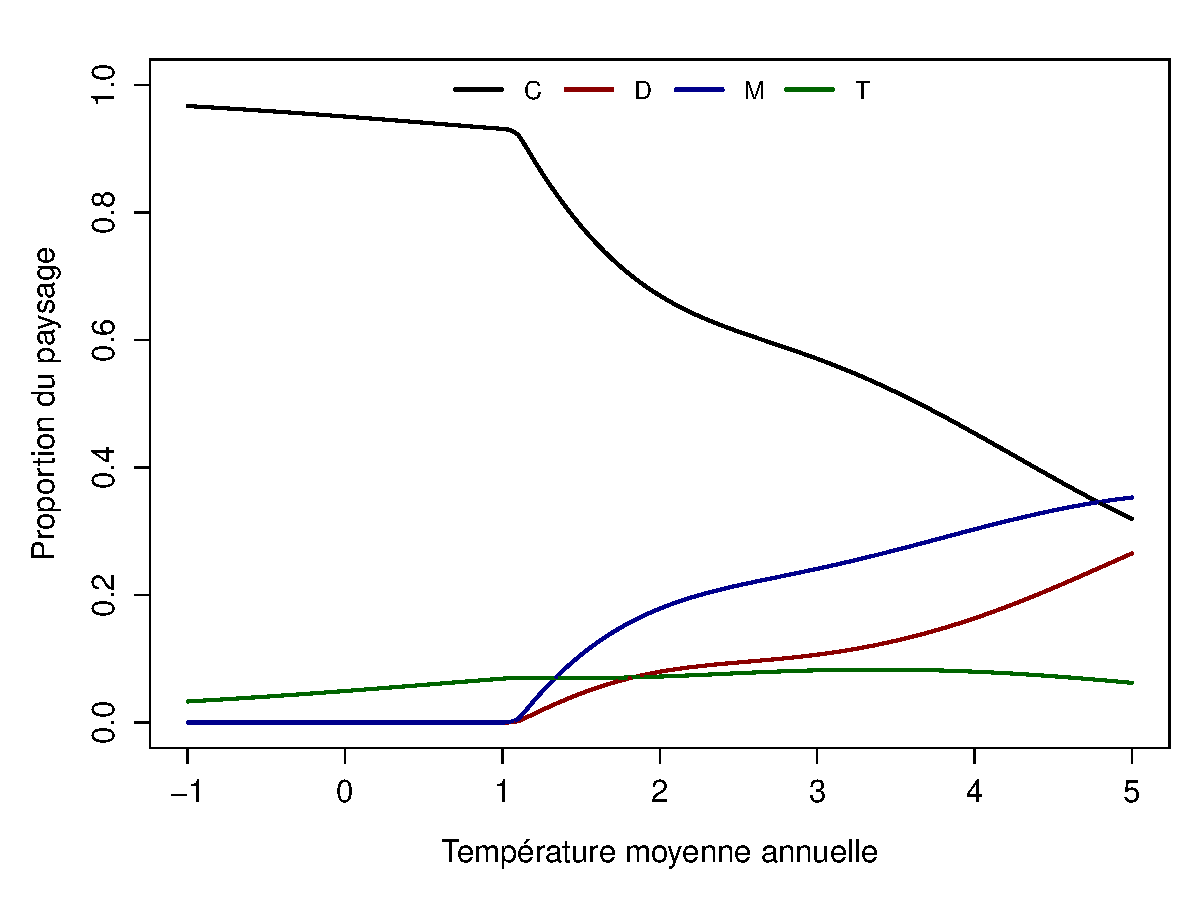
\includegraphics[height=0.4\textheight]{SDMeq}
				\end{center}
			\end{column}
		\end{columns}	    	
	\end{frame}

%-------------------------------------------------------------------------------
%
%	\begin{frame}{Transitions}
%		\begin{center}
%			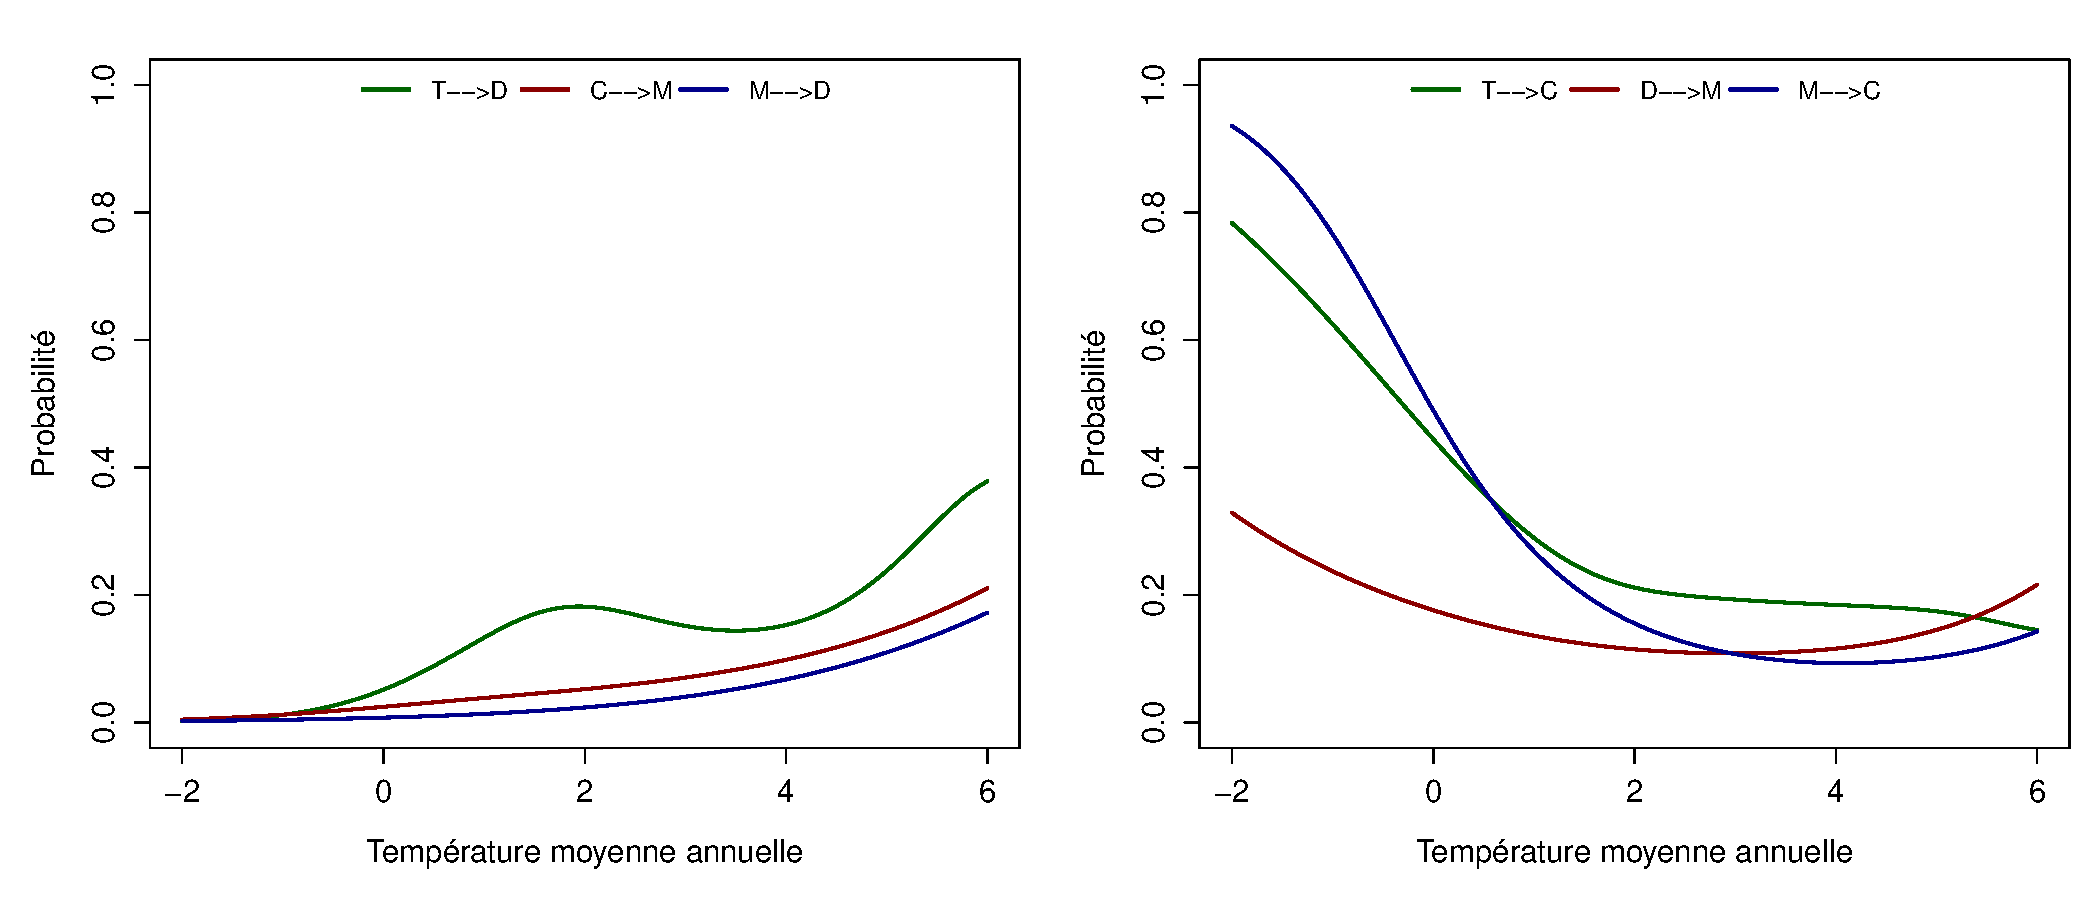
\includegraphics[height=0.5\textheight]{Transitions}
%		\end{center}
%	\end{frame}
%
%-------------------------------------------------------------------------------



	\begin{frame}{Et si on monte la température...}
		\begin{columns}
			\begin{column}{0.5\textwidth}
				\begin{center}
					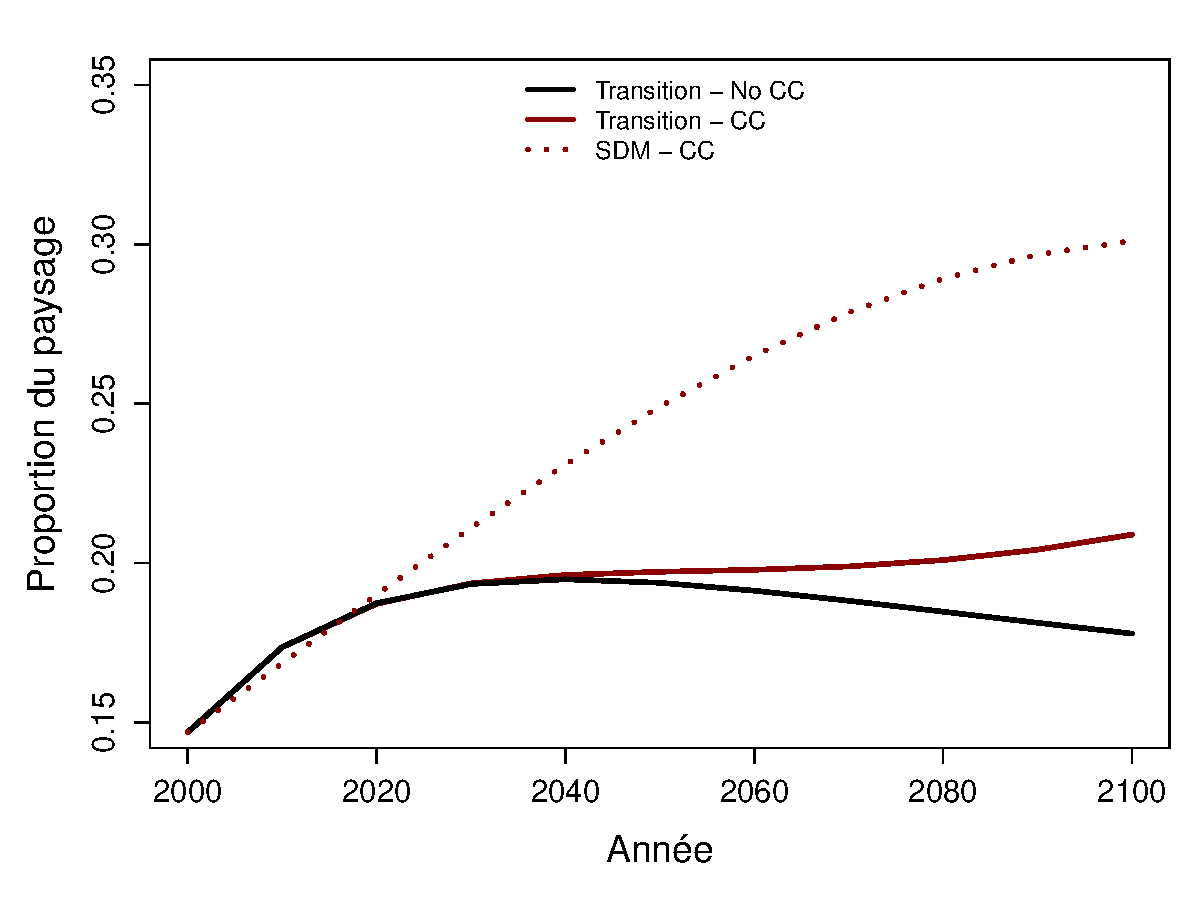
\includegraphics[height=0.5\textheight]{CC_MF}
				\end{center}
			\end{column}
%----
			\begin{column}{0.5\textwidth}
				\begin{itemize}
					\item La distribution actuelle n'est pas nécessairement à l'équilibre;
					\item Intertie énorme de nos forêts;
					\item La dispersion ralentira davantage la réponse;
					\item Une tension entre la végétation potentielle et réalisée s'accumulera avec le temps;
					\item L'écart sera maximal dans la limite entre forêt mixte et forêt boréale.
				\end{itemize}
			\end{column}
		\end{columns}	
	\end{frame}

%-------------------------------------------------------------------------------

	\begin{frame}{Sur une carte}
		\begin{columns}
			\begin{column}{0.25\textwidth}
				\begin{center}
					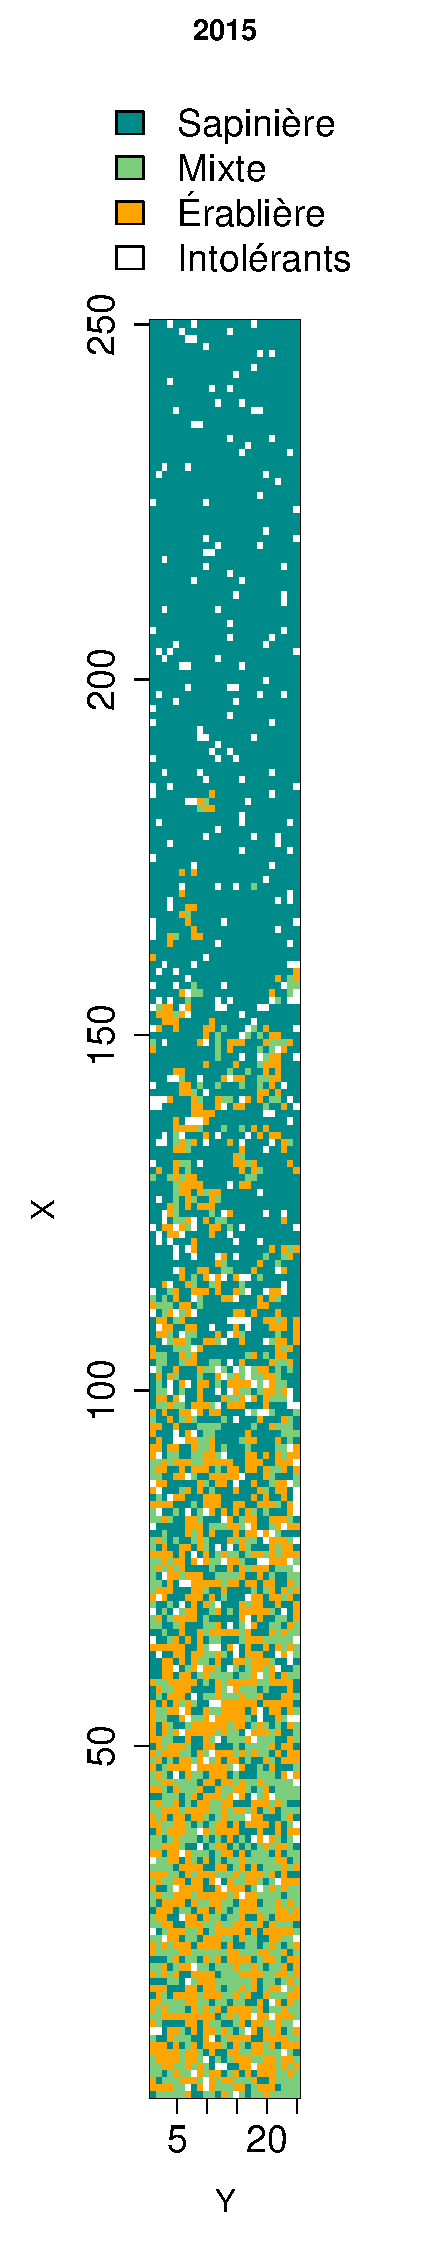
\includegraphics[height=0.8\textheight]{largeplot_2015}
				\end{center}	
			\end{column}
%----
			\begin{column}{0.25\textwidth}
				\begin{center}
					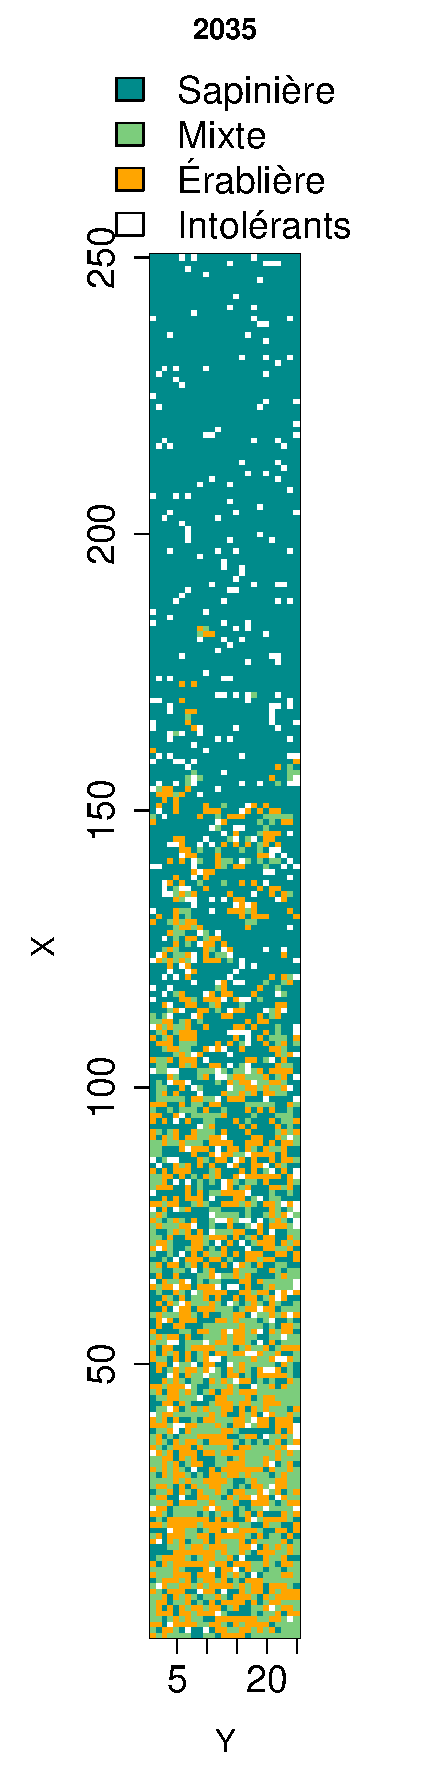
\includegraphics[height=0.8\textheight]{largeplot_2035}
				\end{center}	
			\end{column}
%----
			\begin{column}{0.25\textwidth}
				\begin{center}
					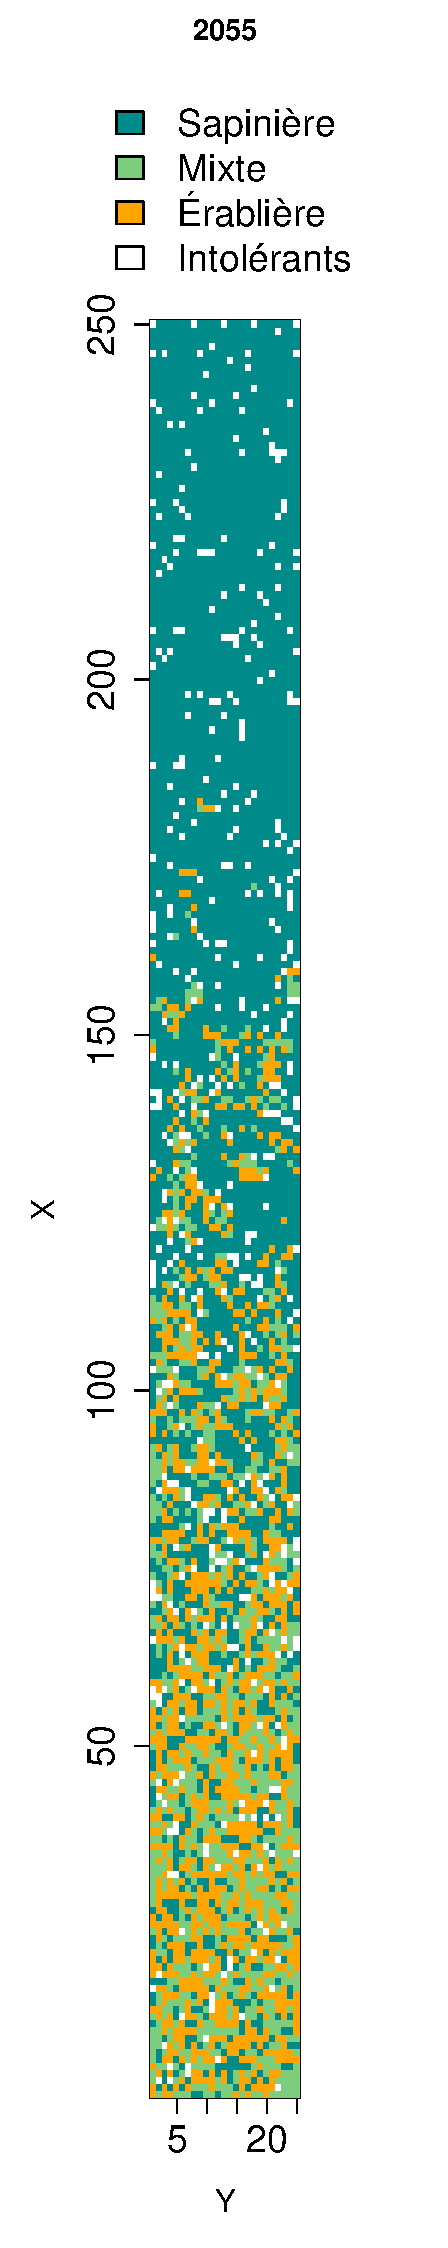
\includegraphics[height=0.8\textheight]{largeplot_2055}
				\end{center}	
			\end{column}
%----
			\begin{column}{0.25\textwidth}
				\begin{center}
					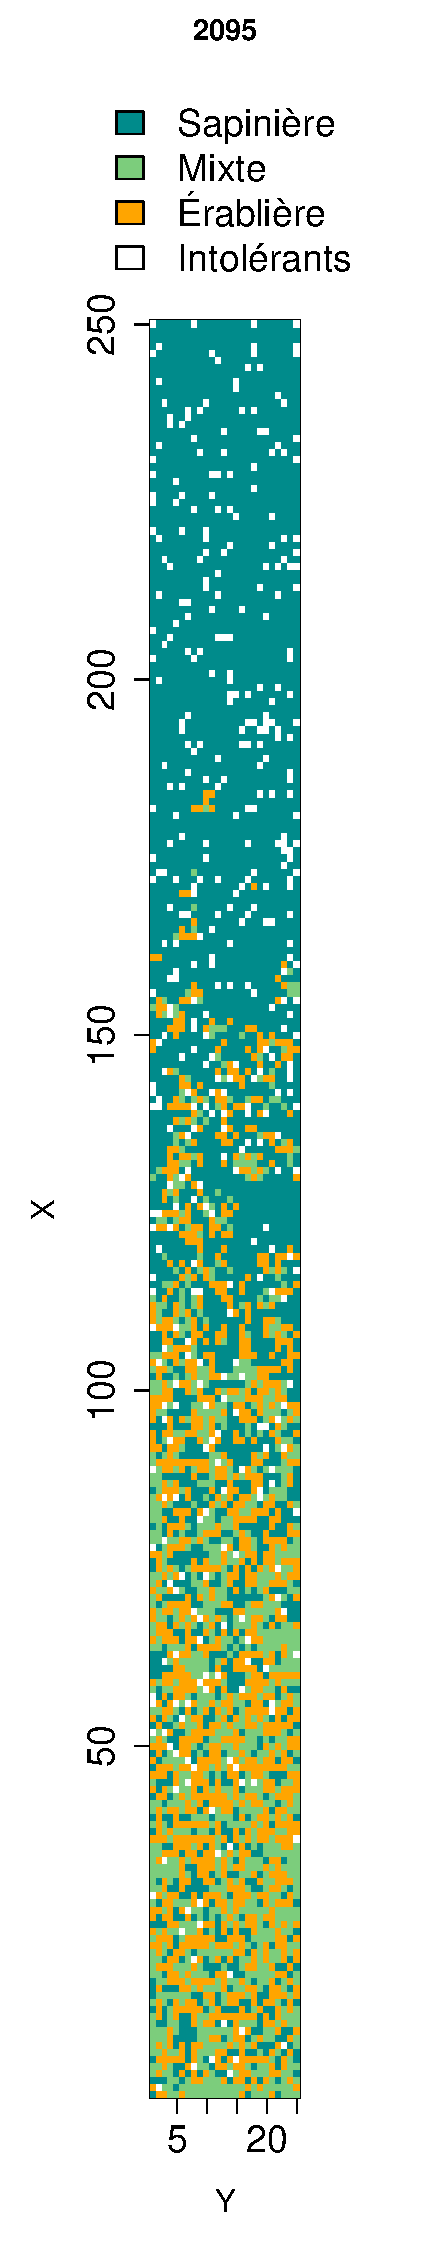
\includegraphics[height=0.8\textheight]{largeplot_2095}
				\end{center}	
			\end{column}						
		\end{columns}	    
	\end{frame}

%-------------------------------------------------------------------------------

%
%	\begin{frame}{Et sur le Pic Champlain}
%		\begin{columns}
%			\begin{column}{0.5\textwidth}
%				Distribution actuelle des états
%				\begin{center}
%					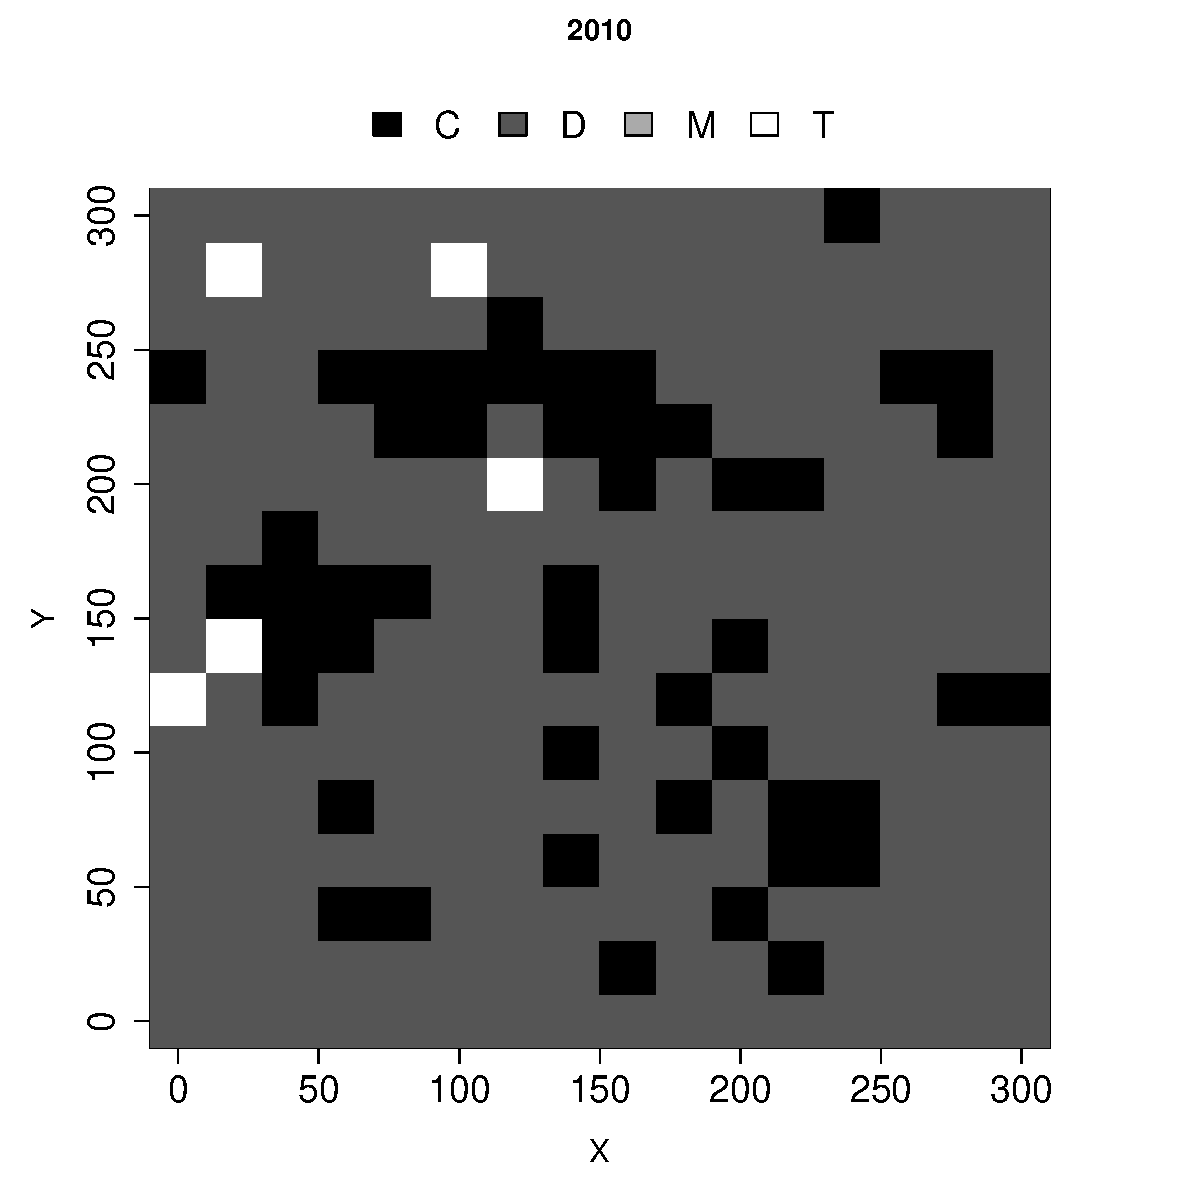
\includegraphics[height=0.5\textheight]{BIC2010}
%				\end{center}
%			\end{column}
%%----
%			\begin{column}{0.5\textwidth}
%
%				
%			\end{column}
%		\end{columns}	    	
%	\end{frame}
%%-------------------------------------------------------------------------------
%
%	\begin{frame}{Et sur le Pic Champlain}
%		\begin{columns}
%			\begin{column}{0.5\textwidth}
%				Distribution actuelle des états
%				\begin{center}
%					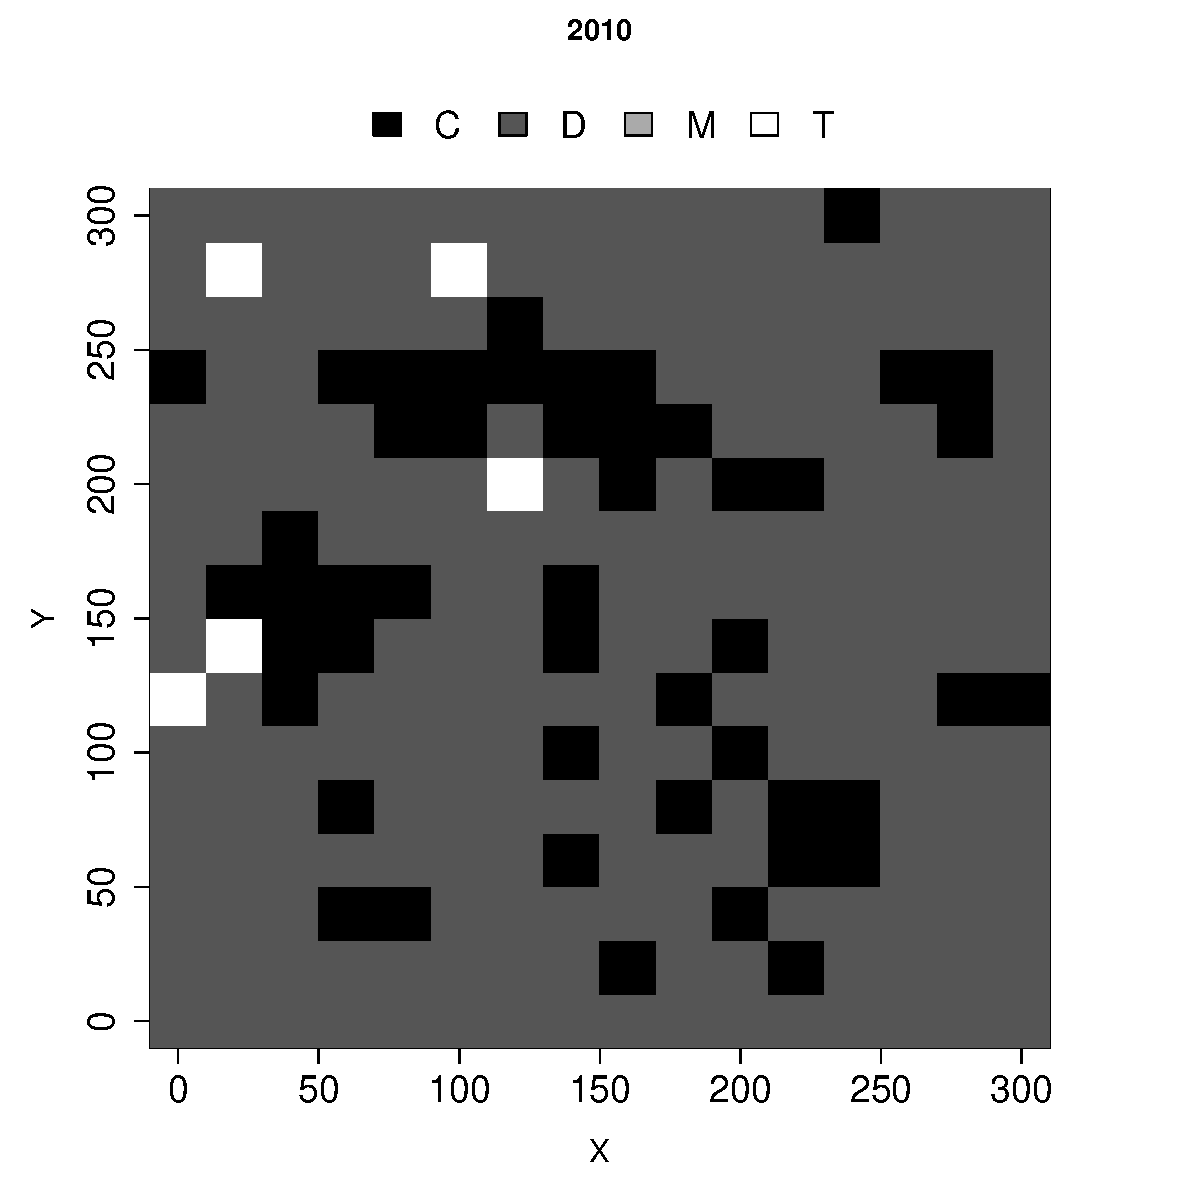
\includegraphics[height=0.5\textheight]{BIC2010}
%				\end{center}
%			\end{column}
%%----
%			\begin{column}{0.5\textwidth}
%				Distribution modélisée
%				\begin{center}
%					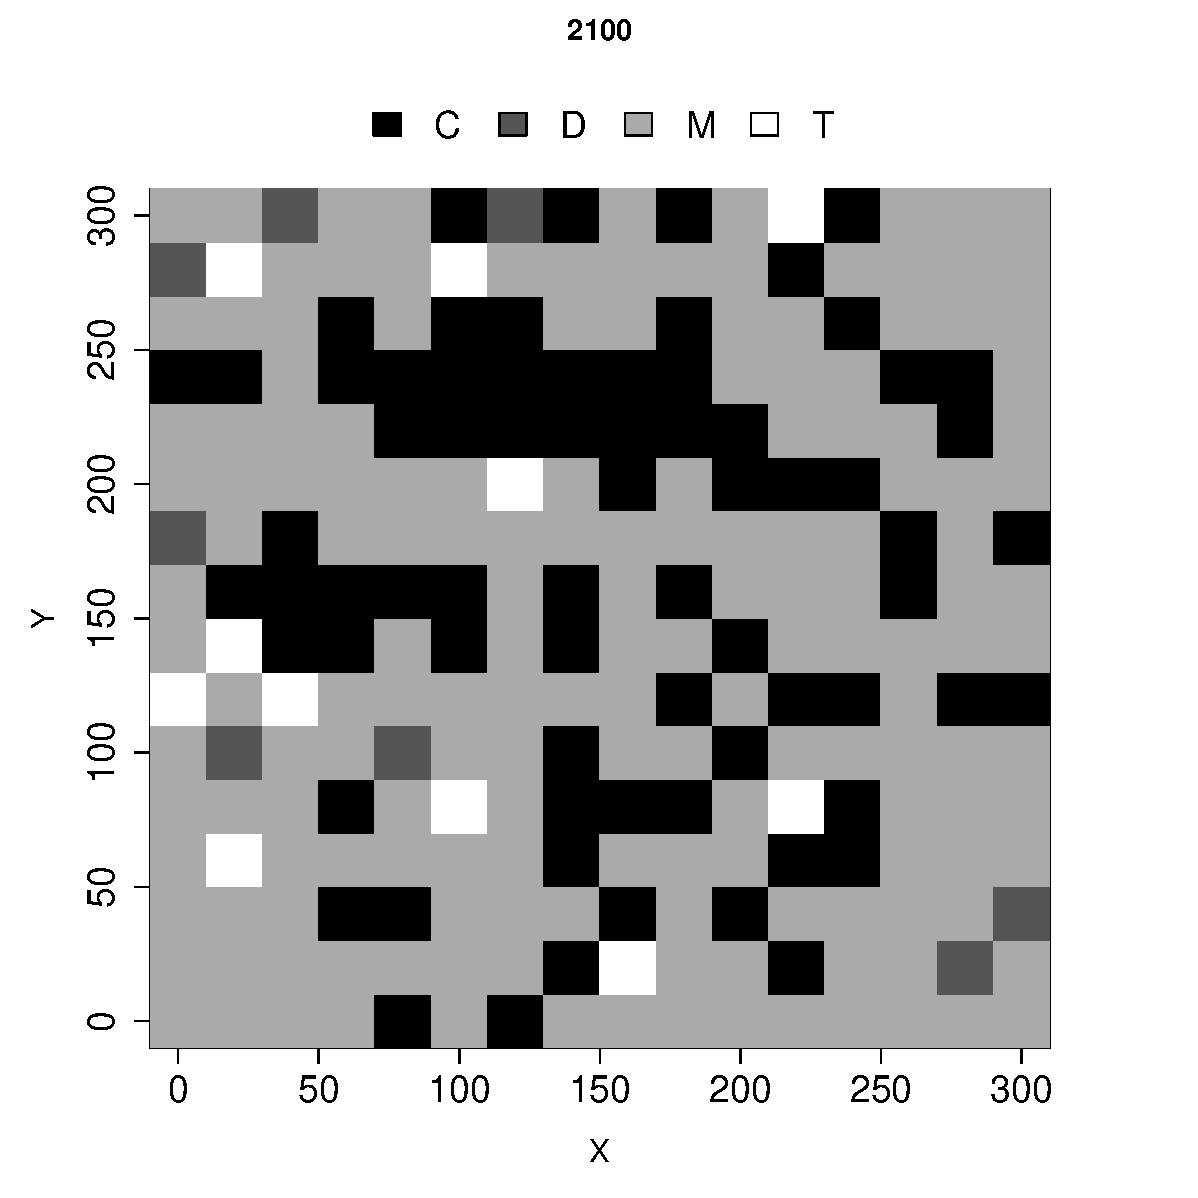
\includegraphics[height=0.5\textheight]{BIC2100}
%				\end{center}
%			\end{column}
%		\end{columns}	    	
%	\end{frame}
%	
%%-------------------------------------------------------------------------------
%-------------------------------------------------------------------------------
\section{Discussion}
%-------------------------------------------------------------------------------
%-------------------------------------------------------------------------------

	\begin{frame}{Discussion}{Changements abruptes et aménagement écosystémique?}
		\begin{columns}
			\begin{column}{0.5\textwidth}
				\begin{center}
				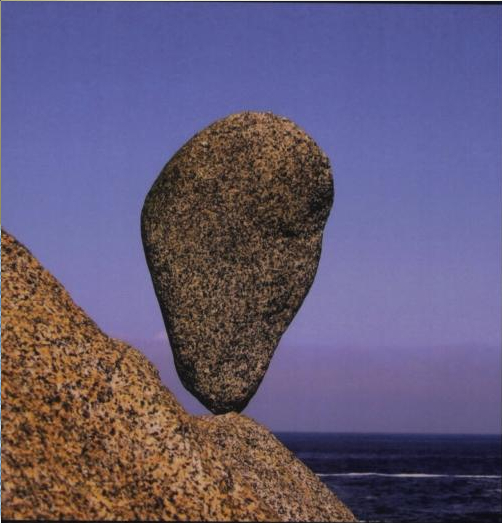
\includegraphics[height=0.6\textheight]{scheffer}\\
				\end{center}
			\end{column}
%----
			\begin{column}{0.5\textwidth}
				\begin{itemize}
				\item Distribution bimodale de l'abondance de la forêt décidue;
				\item Relation non-linéaire entre abondance de la forêt décidue et température;
				\item Distribution qui n'est pas à l'équilibre;
				\item Résistance au réchauffement climatique (augmentation des écarts);
				\item Effet de la structure spatiale.
				\end{itemize}
			\end{column}
		\end{columns}	
	\end{frame}

%-------------------------------------------------------------------------------

	\begin{frame}{À venir}
		\begin{itemize}
			\item Étude expérimentale de la germination;
			\item Formulation et intégration d'un modèle démographique;
			\item Étude des vitesses de migration;
			\item Étude de la productivité;
			\item Modèle épidémiologique pour la TBE;
			\item Ajout de l'aménagement forestier.
		\end{itemize}
	\end{frame}

%------------------------------

	\begin{frame}{Livrables}
		\begin{itemize}
			\item Cartes de distribution des espèces;
			\item Cartes de changement de productivité;
			\item Version ''user-friendly'' du modèle et formation;
			\item Évaluation stratégique de scénarios d'aménagement forestier.
		\end{itemize}
	\end{frame}

%-------------------------------------------------------------------------------


	\begin{frame}{Collaborateurs}

	\textbf{Chercheurs:} Robert Schneider, Luc Sirois, Dominique Arseneault, Yves Bergeron, Christian Messier, Frédéric Doyon, Igor Drobyshev, Osvaldo Valeria, Marie-Josée Fortin\\ 
	\vskip 1em        	    	    
	\textbf{Étudiants} Steve Vissault, Matt Talluto, Isabelle Boulangeat, Kevin Solarik, Alyssa Butler, Lise Jaton, Raphael Aussenac, Hedvig Nenzen;\\ 
	\vskip 1em
	\textbf{Partenaires:} Parc national du Bic, CRÉ Bas-St-Laurent, Domtar, Tembec, Produits forestiers Résolu, SCF, MRN, Nature Conservancy, Corridor Appalachien;
	\vskip 1em
	\textbf{Financement:} FRQNT, CRSNG, Chaires de recherche du Canada, Tembec, CSBQ, CEF.

	\end{frame}

%------------------------------

%------------------------------
\end{document}
